\section{Introduction to Reinforcement Learning}
Learning from interaction is an idea that is at the basis of nearly all theories of learning and intelligence, among which we find reinforcement learning.

Reinforcement learning is learning what to do and how to map situations to actions, so as to maximize a numerical reward (it is goal-directed learning from interaction). The learner is not told which actions to take, but instead it must discover which actions yield the most reward by trying them. In the most interesting and challenging cases, actions may affect not only the immediate reward but also the next situation and, through that, all subsequent rewards. These two characteristics (trial-and-error search and delayed reward) are the two most important distinguishing features of reinforcement learning.

We will now introduce finite Markov decision processes, a mathematical framework that we are going to use.

\subsection{Finite Markov Decision Processes}
Markov Decision Processes (MDPs) are a mathematically idealized formulation of reinforcement learning for which precise theoretical statements can be made. They provide a mathematical framework for modeling decision making in situations where outcomes are partly random and partly under the control of a decision maker\footnote{See \url{https://en.wikipedia.org/wiki/Markov_decision_process}}.

At each time step $t$, the process is in some state $s$, and the decision maker may choose an action $a$ that is available in state $s$. The process responds at the next time step by randomly moving into a new state $s'$, and giving the decision maker a corresponding reward $R_a(s,s')$. The probability that the process moves into its new state $s'$ is influenced by the chosen action. Specifically, it is given by the state transition function $P_a(s,s')$. Thus, the next state $s'$ depends on the current state $s$ and the decision maker's action $a$. But \textbf{given $s$ and $a$, it is conditionally independent of all previous states and actions}; in other words, the state transitions of an MDP satisfy the Markov property \textit{(memoryless property of a stochastic process)}.

\begin{figure}[hbt]
    \centering
    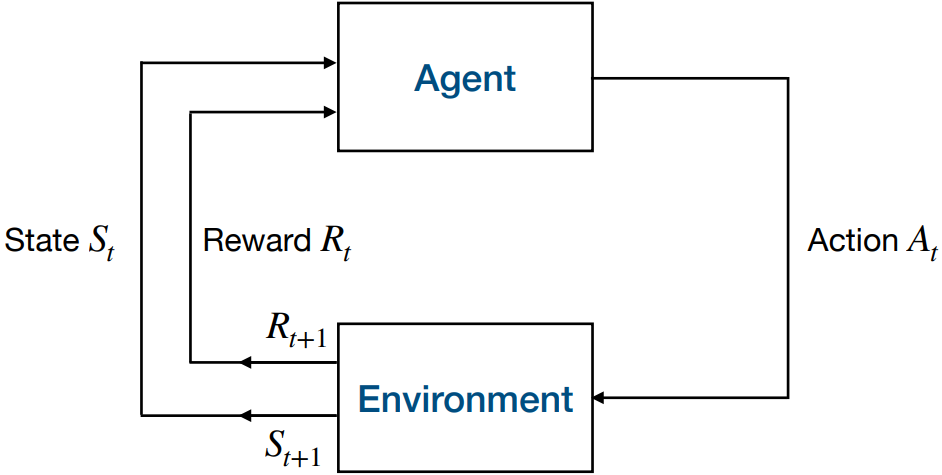
\includegraphics[width=\textwidth]{Images/Chapter 2/mdp.png}
    \caption{Schema of a Markov Decision Process.}
    \label{fig:ch2-mdp}
\end{figure}

\subsection{Rewards and expected returns}
Informally, the agent’s goal is to maximize the \textbf{total amount} of rewards it receives (note how the agent should not maximize the immediate reward, but the cumulative reward). We can formalize this with the \textbf{``reward hypothesis''}: \textit{``That all of what we mean by goals and purposes can be well thought of as the maximization of the expected value of the cumulative sum of a received scalar signal (called reward)''}.

We will now try to conceptualize the idea of \textbf{cumulative rewards} more formally by means of the notion of \textbf{expected return} $G_t$. To do so, we first need to distinguish between two cases:
\begin{itemize}
    \item \textbf{Episodic tasks}, in which we can identify a final step of the sequence of rewards (i.e., in which the interaction between the agent and the environment can be broken into sub-sequences called \textbf{episodes}, such as playing a game, repeated tasks, etc.). Each episode ends in a terminal state after $T$ steps, followed by a reset to a standard starting state or to a sample of a distribution of starting states (the next episode will be completely independent from the previous one).
    \item \textbf{Continuous tasks}, in which the agent-environment interaction does not break naturally into identifiable episodes, but goes on continually without limit (e.g., an ongoing monitoring of a process).
\end{itemize}

The expected return $G_t$ associated to the selection of an action $A_t$, assuming that the agent receives over time a sequence of rewards $R_{t+1}, R_{t+2}, R_{t+3}, ...$ is defined as:
\begin{itemize}
    \item The sum of the future rewards \textbf{in the case of episodic tasks}:
    \begin{equation}
        G_t \doteq R_{t+1} + R_{t+2} + R_{t+3} + ... + R_t
        \label{eq:ch2-expectedreturn-episodic}
    \end{equation}
    \item The weighted sum of the future rewards \textbf{in the case of continuing tasks}:
    \begin{equation}
        G_t \doteq R_{t+1} + \gamma R_{t+2} + \gamma^2 R_{t+3} + ... = \sum_{k=0}^{\infty} \gamma^k R_{t+k+1}
        \label{eq:ch2-expectedreturn-continuous}
    \end{equation}
\end{itemize}

Where $\gamma$ is the \textbf{discount rate}, with $0 \le \gamma \le 1$. The discount rate is used to give more importance to the rewards that are closer to us in time; this is particularly useful in dynamic environments. The definition of expected return that we used for episodic tasks would in fact be problematic for continuing tasks: the expected return at the time of termination $T$ would be equal to $\infty$ in some cases, such as when the reward is equal to $1$ at each time step. The discount rate determines the ``present value of future rewards'' (how much future rewards mean to us at the current time): a reward received $k$ time steps in the future is worth $\gamma^{k-1}$ of what it would be worth if it were received immediately.

Returns at successive time steps are related to each other as follows:
\begin{equation*}
    \begin{split}
        G_t & \doteq R_{t+1} + \gamma R_{t+2} + \gamma^2 R_{t+3} + \gamma^3 R_{t+4} + ... \\
        & = R_{t+1} + \gamma \left( R_{t+2} + \gamma R_{t+3} + \gamma^2 R_{t+4} + ... \right) \\
        & = R_{t+1} + \gamma G_{t+1} \\
    \end{split}
\end{equation*}

\subsection{Policies and value functions}
Almost all reinforcement learning algorithms involve estimating value functions, i.e., functions of states (or of state-action pairs) that estimate how good it is for the agent to be in a given state (or how good it is to perform a given action in a given state). The notion of ``how good'' here is defined in terms of future rewards that can be expected, or, to be precise, in terms of expected return.

A \textbf{policy} is used to model how the agent will behave based on the previous experience and the rewards (and, consequently, the expected returns) an agent received in the past. Formally, a policy is a mapping from states to probabilities of each possible action (the probability of taking a certain action in a certain state). If the agent is following the policy $\pi$ at time $t$, then $\pi (a \vert s)$ is the probability that $A_t=a$ if $S_t=s$.

\textbf{The value function of a state s under a policy $\pi$}, denoted $v_\pi (s)$, is the expected return when starting in $s$ and following $\pi$ thereafter (the expected return I can have in the future state, considering all the actions I might take from there). For Markov Decision Processes, we can define \textbf{the state-value function} $v_\pi$ for the policy $\pi$ formally as:
\begin{equation}
    v_s \doteq \mathbb{E}_\pi \left[ G_t  \ \vert \  S_t = s \right] = \mathbb{E}_\pi \left[ \sum_{k=0}^{\infty}  \gamma^k R_{t+k+1} \  \middle\vert \  S_t = s, A_t = a \right] \quad \forall s \in \mathcal{S}
    \label{eq:ch2-statevaluefunction}
\end{equation}

Where $\mathbb{E}_\pi [\cdot]$ denotes the expected value of a random variable given that the agent follows $\pi$ and $t$ is any time step. Note that the value of the terminal state, if any, is always $0$. The formula above denotes a weighted average of the expected value (it is averaged because the values depend on the probability of a certain action being taken, which is a fraction).

Similar to what we just did, we can define \textbf{the action-value function}, i.e., the value of taking an action $a$ in the state $s$ under a policy $\pi$, denoted $q_\pi (s,a)$, as the expected return starting from $s$, taking the action $a$, and following the policy $\pi$ thereafter:
\begin{equation}
    q_\pi(s,a) \doteq \mathbb{E}_\pi \left[ G_t \  \vert \  S_t = s, A_t = a \right] = \mathbb{E}_\pi \left[ \sum_{k=0}^{\infty} \gamma^k R_{t+k+1} \  \middle\vert \ S_t = s, A_t = a \right]
    \label{eq:ch2-actionvaluefunction}
\end{equation}

\subsection{Choosing the rewards}
When we model a real system as a reinforcement learning problem, the most difficult task is selecting the right rewards. Typically, we use negative values for actions that do not help us in reaching our goal, and positive if they do (it is also possible using 0 as a value for actions that do not help us). An alternative is to set the values of the rewards to a negative number until we reach our goal (using 0 as the value when we reach it).

When choosing the rewards, it is very important that \textbf{we should not ``reward'' the intermediate steps or the single actions}. The agent, in fact, always learns to maximize its reward. If we want it to do something for us, we must provide rewards to it in such a way that in maximizing them the agent will also achieve our goals. It is thus critical that the rewards we set up truly indicate what we want accomplished. If we were to give importance to certain sub-goals, the agent might find a way to achieve them without achieving the real goal (e.g., taking the opponent's pieces while playing chess but losing the game). Note that the reward signal is our way of communicating to the agent \textit{what} we want achieved, not \textit{how} (a better place for imparting this kind of prior knowledge would be the initial policy or the initial value function).

Giving rewards to the agent could be a challenging task, as we will see from the two examples that follow. Let us first imagine that we want to create an agent that completes a maze in the least time possible: we could give a reward of -1 for every step it takes inside the maze and 0 for reaching the exit. This could work even if we assume that we only have one episode to base our rewards on. There are situations, though, in which we need additional information to quantify how good an action is for us, like in a game of chess, where we can only assign the rewards at the end of the game (e.g., assigning 1 to every step if we won, -1 if we lost). This is usually called \textbf{credit assignment problem} (i.e., the problem of assigning a reward to each step) and a discussion on it can be found in Marvin Minsky’s ``Steps Towards Artificial Intelligence'' paper \cite{4066245}.

We now need to think about how we can solve this problem and estimate the value functions $v_\pi$ and $q_\pi$. If the behavior of the Markov Decision Process is known (i.e., the transition probabilities between all the states are known), we could do so by considering all the possible moves, although this poses strict requirements in terms of prior knowledge and system complexity. A more general option is to estimate them through experience: if an agent follows policy $\pi$ and maintains an average, for each state encountered, of the actual returns that have followed that state, then the average will converge asymptotically to the state’s value, $v_\pi(s)$, as the number of times that state is encountered approaches infinity (these methods are referred to as \textbf{Monte Carlo methods} because they involve averaging over many random samples of actual returns). This option is still problematic when it comes to very large number of states, though, as it would involve keeping separate averages for each state individually. In those cases, instead, we will maintain $v_\pi$ and $q_\pi$ as parametrized functions, with fewer parameters than the number of states, using approximators such as artificial neural networks.

\subsection{Optimal policies and optimal value functions}
Solving a reinforcement learning task is roughly equivalent to finding a policy that maximizes the amount of reward over the long run. In finite Markov Decision Processes, there is always at least one policy $\pi$ that is better than or equal to all the other policies, meaning that its expected return is greater than or equal to that of a different policy $\pi'$ for all states. More formally:
\begin{equation*}
    \pi \ge \pi' \text{ if and only if } v_\pi(s) \ge v_{\pi'} (s) \quad \forall s \in \mathcal{S}
\end{equation*}

Although there may be more than one, we denote all the optimal policies with $\pi_*$. They share the same state-value function, called the \textbf{optimal state-value function}, denoted $v_*$ and defined as:
\begin{equation}
    v_*(s) \doteq \max_\pi v_\pi(s) \quad \forall s \in \mathcal{S}
    \label{eq:ch2-optimalstatevaluefunction}
\end{equation}

This means that, given a state and the value function, the optimal policy is the one that gives us the maximum reward. The same goes for the \textbf{optimal action-value function}, denoted $q_*$ and defined as:
\begin{equation}
    q_*(s,a) \doteq \max_\pi q_\pi(s,a) \quad \forall s \in \mathcal{S}, a \in \mathcal{A}(s)
    \label{eq:ch2-optimalactionvaluefunction}
\end{equation}

For the state-action pair $(s,a)$, this function gives the expected return for taking the action $a$ in the state $s$ and thereafter following an optimal policy. Thus, we can write $q_*$ in terms of $v_*$ as follows:
\begin{equation*}
    q_*(s,a) = \mathbb{E} \left[ R_{t+1} + \gamma v_* S_{t+1} \  \middle\vert \ S_t = s, A_t = a \right]
\end{equation*}

\subsection{Optimality and approximation}
\subsubsection{Bellman equation}
What we are doing is closely related to the issues of automatic control: we both want to have knowledge and control over the evolution of a system.

For any policy $\pi$ and any state $s$, the following consistency condition holds between the value of $s$ and the value of its possible successor states:
\begin{equation}
    \begin{split}
        v_\pi(s) & \doteq \mathbb{E}_\pi \left[ G_t \ \vert \ S_t = s \right] \\
        & = \mathbb{E}_\pi \left[ R_{t+1} + \gamma G_{t+1} \ \vert \ S_t = s \right] \\
        & = \sum_{a} \pi(a \vert s) \sum_{s'} \sum_{r} p(s',r \ \vert \ s,a) \Big[ r + \gamma \mathbb{E}_\pi \left[ G_{t+1} \ \vert \ S_{t+1} = s' \right] \Big] \\
        & = \sum_{a} \pi (a \vert s) \sum_{s', r} p(s', r \ \vert \ s,a) \Big[ r + \gamma v_\pi(s') \Big], \quad \forall s \in \mathcal{S}
    \end{split}
    \label{eq:ch2-bellmanequation}
\end{equation}

What we have in the end is known as the \textbf{Bellman equation} for $v_\pi$ and it states that the value of the start state must equal the (discounted) value of the expected next state, plus the reward expected along the way.

\subsubsection{Bellman optimality equation}
We can re-write the Bellman equation under the optimal policy, obtaining what is known as the \textbf{Bellman optimality equation}:
\begin{equation}
    \begin{split}
        q_*(s,a) & = \mathbb{E} \left[ R_{t+1} + \gamma \max_{a'} q_* (S_{t+1}, a') \ \middle\vert \ S_t = s, A_t = a \right] \\
        & = \sum_{s', r} p(s',r \ \vert \ s,a) \left[ r + \gamma \max_{a'} q_*(s',a') \right]
    \end{split}
    \label{eq:ch2-bellmanoptimalityequation}
\end{equation}

Intuitively, the Bellman optimality equation must equal the expected return for the best action from that state. 

The Bellman optimality equation is actually a system of equations, one for each state, so if there are $n$ states, then there are $n$ equations in $n$ unknowns. If the dynamics $p$ of the environments are known, then in principle one can solve this system of equation for $v_*$. Once we have $v_*$ (or $q_*$), the actions that select the highest value for them in each state will then be the optimal actions. Another way of saying this is that any policy that is \textbf{greedy} with respect to the optimal evaluation function is an optimal policy. As a reminder, the term \textit{greedy} is used in computer science to describe any search or decision procedure that selects alternatives based only on local or immediate considerations, without considering the possibility that such a selection may prevent future access to even better alternatives. This is not an issue in the case of Markov Decision processes, though, as they indeed depend only on the current state: \textbf{a greedy policy is then optimal both in the short and in the long-term}.

As we were hinting at earlier, it may not always be possible to solve the Bellman optimality equations, both due to the huge number of states (and equations) involved in non-trivial problems and because the state may not be fully observable, or we may not be able to know its dynamics.

\subsection{Differences between Reinforcement Learning and other types of learning}
As the last thing in this chapter, we try to make sure we have a clear idea of the differences between reinforcement learning and other types of learning and how it constitutes a third paradigm for learning.

\subsubsection{Reinforcement learning vs Supervised learning}
Supervised learning mainly deals with classification: being able to map a certain vectorial input to a set of labels. The supervised algorithms learn by being ``fed'' labelled examples that must be representative of runtime inputs to work: this clashes with the typical reinforcement learning application scenario of unknown situations.

\subsubsection{Reinforcement learning vs Unsupervised learning}
Unsupervised learning deals with information provided in unlabeled datasets and tries to find patterns, typically by means of clustering based on a distance function. Reinforcement learning, despite not relying on labels of correct behavior like unsupervised learning, has the goal of maximizing a reward signal instead of trying to find a hidden structure in a dataset.